\section{Conclusion}
\label{sec:conclusion}

\par To better understand the similarities and also what differs most in the results using the theoretical and simulated analysis, the tables with the important values are given side by side:

\begin{table}[ht]
\parbox{.55\linewidth}{
  \centering
  \begin{tabular}{|l|r|}
    \hline    
    {\bf Name} & {\bf Value} \\ \hline
    $Gain Deviation [V]$ & 1.340000e+00 \\ \hline 
$Central Frequency Deviation [Hz]$ & 2.308672e+01 \\ \hline 
$Cost$ & 1.352633e+04 \\ \hline 
$Merit$ & 3.026597e-06 \\ \hline 

  \end{tabular}
  \caption{Obtained results using Octave}} 
\parbox{.55\linewidth}{
 \centering
  \begin{tabular}{|l|r|}
    \hline    
    {\bf Name} & {\bf Value} \\ \hline
    \input{../sim/results_tab}
  \end{tabular}
  \caption{Obtained results using NGSpice}}
\end{table}

\par Taking a closer look at these values, one notices that there are some discrepancies. These differences have a direct consequence in the value of the merit, since it depends on these quantities. However, one notices that the theoretical merit does not differ that much from the simulated one. 
\par The differences between the analysis were expected and could be caused due to the aproximations made during the theoretical analysis while Ngspice uses much more complex models to predict the same quantities, since some of the components of the circuit are not linear.
\par Looking at the values for the impedances shown in the previous sections ~\ref{sec:analysis} and ~\ref{sec:simulation}, one sees a few discrepancies, due to, once again, the ideal models used in the theoretical analysis that are much simpler than the ones used in the simulation tool.
\par Looking at the gain and central frequency deviations in both analysis, one concludes that these values are very satisfactory, since they do not differ much from the values given by the teacher prior to the lab assignment.
\par In fact, the value for the merit is quite small since the cost of this circuit is very big, mainly because of the OP-AMP. Taking that into consideration, the obtained values were within the expected.
\par As usual, the merit to take into consideration is the simulated one, since $Ngspice$ has the ability to produce values that are much more similar to reality.
\par It is also important to compare the graphics obtained in both methods(see below), since they give valuable information to compare the results. One sees that the curves represented are very similar, both in the frequency analysis of the gain and the phase, which leads us to conclude that the these figures were well produced and the theory behind them is correct.

\begin{figure}[ht]
\centering
\parbox{.47\linewidth}{
  \centering
  \includegraphics[width=.7\linewidth]{gain.eps}
  \caption{Gain [dB] using Octave}
  \label{fig:matfg} }
\parbox{.47\linewidth}{
  \centering
  \includegraphics[width=.65\linewidth]{vo1f.pdf}
  \caption{Gain [dB] using Ngspice}
  \label{fig:simfg}}
\end{figure}

\begin{figure}[ht]
\centering
\parbox{.47\linewidth}{
  \centering
  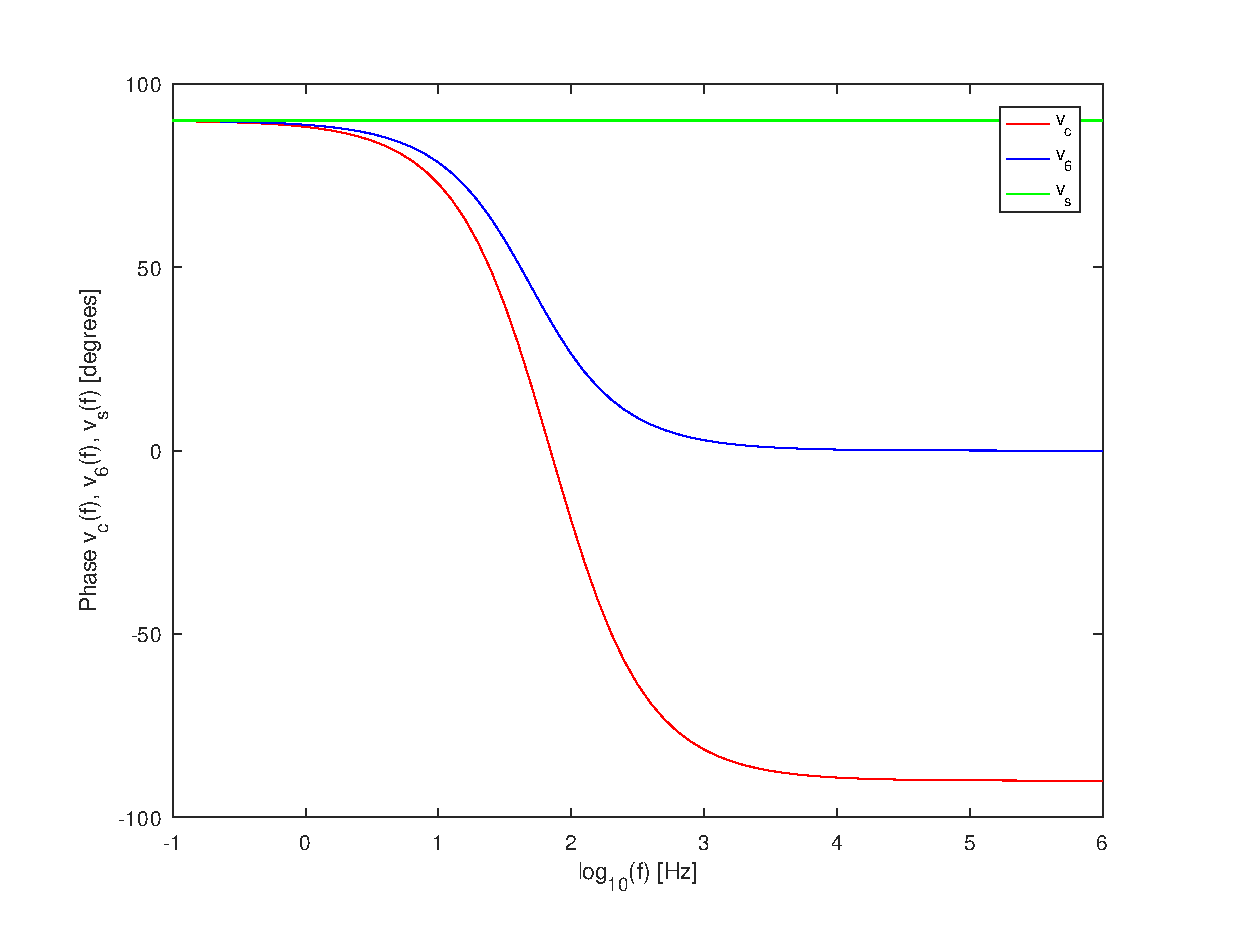
\includegraphics[width=.7\linewidth]{phase.eps}
  \caption{Phase [degrees] using Octave}
  \label{fig:matfp} }
\parbox{.47\linewidth}{
  \centering
  \includegraphics[width=.65\linewidth]{vo2f.pdf}
  \caption{Phase [degrees] using Ngspice}
  \label{fig:simfp}}
\end{figure}

\par In conclusion, although there are some differences (that were expected), the objective of this lab assignment was accomplished and both methods (theoretical end simulated) were able to filter the unwanted frequencies, both very low and very high.
